
%%%%% <standalone preamble
\documentclass[]{article}

\usepackage{graphicx}
\usepackage{bm}
\usepackage{amsfonts} %for mathbb?
\usepackage{amsmath} 
%\usepackage{caption}

\graphicspath{{./Chapter_4_Fig/}}
%%%%%% />
%=== Chapter Four ===
%\chapter{Intersection Control for Automated Vehicles }

%%%%% </standalone preamble> 
\title{Intersection Control for Automated Vehicles }
\author{Edward Lambert}
\begin{document}
\maketitle
\begin{abstract}
\end{abstract}
%%%%% <standalone preamble/>


\section{Introduction}
The capacity and safety of an intersection can be considered in terms of the number and type of conflict points which it contains. When every entrance to the intersection is connected to every exit by a smooth arc, a conflict point exists wherever two arcs intersect. They can be classified as head-on, following, crossing, diverging or merging. In many studies these points are assumed to be fixed, and only speed of the vehicles which controls the rate of progress along the arcs is varied to minimise delay. 

With the development of path planning around obstacles on-the-fly, it becomes possible to consider what arrangement of conflict points is best given the traffic at a particular instant in the near future. 

%The distributed consensus on the arrival order underpins the distributed solution for trajectory planning. The body of work considering flexible paths for aircraft relies on similar techniques to the latest works targeted at Connected Automated Road Vehicles where the paths are fixed. Specifically \cite{Liu2018} uses sequential per-vehicle optimisation to find the highest safe speeds subject to static obstacle constraints, and the trajectories of vehicles earlier in the sequence. The crossing order is determined by the arrival time at the 'point of no return' according to the motion model of each vehicle. The high frequency closed loop controller on one vehicle continues to operate while the others are formulating their own trajectory plan. Similarly the work on adaptive paths in \cite{Luis2018} uses simultaneous per-vehicle optimisation to find the trajectory as a sequence of control actions and associated positions at regular time intervals which the vehicle is predicted to occupy up to a receding time horizon. Both offer a suboptimal global (all-vehicles) solution, which is guaranteed to be safe. Could the simultaneous approach improve performance of DMPC? Is it just a different name for the same algorithm? An existing constrained optimisation based path planner could be used to generate trajectories by assuming a simple speed profile. Mutual constraints between two trajectories can then be applied, with one constraint for each time sample, leading to a solution to the central(all-vehicle) multi-vehicle trajectory planning problem. The local(per-vehicle) optimization is identical to the global(all-vehicle) one, only the passing order choice need to reach consensus. Either of the two aforementioned decentralized ordering algorithms should be applicable. Which is most promising, resulting in a consensus with the least deviation from central(all-vehicle) optimality? Does the answer change depending on the nature of the path optimisation, should it be based on a clothoid spline or radial polynomials?

 
%==================


\section{Simulation}

Platooning with speed choice by a centralized controller was implemented with a vehicle to intersection messaging scheme. The full site is divided into zones, each one containing a single intersection. Each AGV in the fleet has a copy of the roadmap which is  static. The fleet controller interfaces with the warehouse management system to get the next material transfer job, consisting of a pick location and a drop location. All jobs are assumed to be of unit size and each AGV has a capacity of one unit. With these assumptions, a straightforward policy is to assign the next job to the AGV nearest to the pick location - first-come-first-served scheduling. When an AGV receives a new job, it finds the shortest path through the roadmap using the Floyd-Warshall algorithm \cite{Djojo2013}. Next it must send its planned path to the intersection controller for the zone it currently occupies. The intersection controller stores the plan and current position of every AGV approaching the conflict point of the intersection. Every time it receives a new plan it must recalculate the approach speed for every approaching AGV to minimize total travel time without collision. This will happen every time an AGV enters the zone from somewhere else, or an AGV within the zone is assigned a new job.

%\begin{figure}[ht]
%\centering
%\includegraphics[width=\linewidth]{intersection_layout_trim}
%\caption{Intersection layout shown in SUMO NETEDIT tool \cite{dlr2016}}
%\label{fig:layout}
%\end{figure}
\begin{figure}[ht]
	\centering
	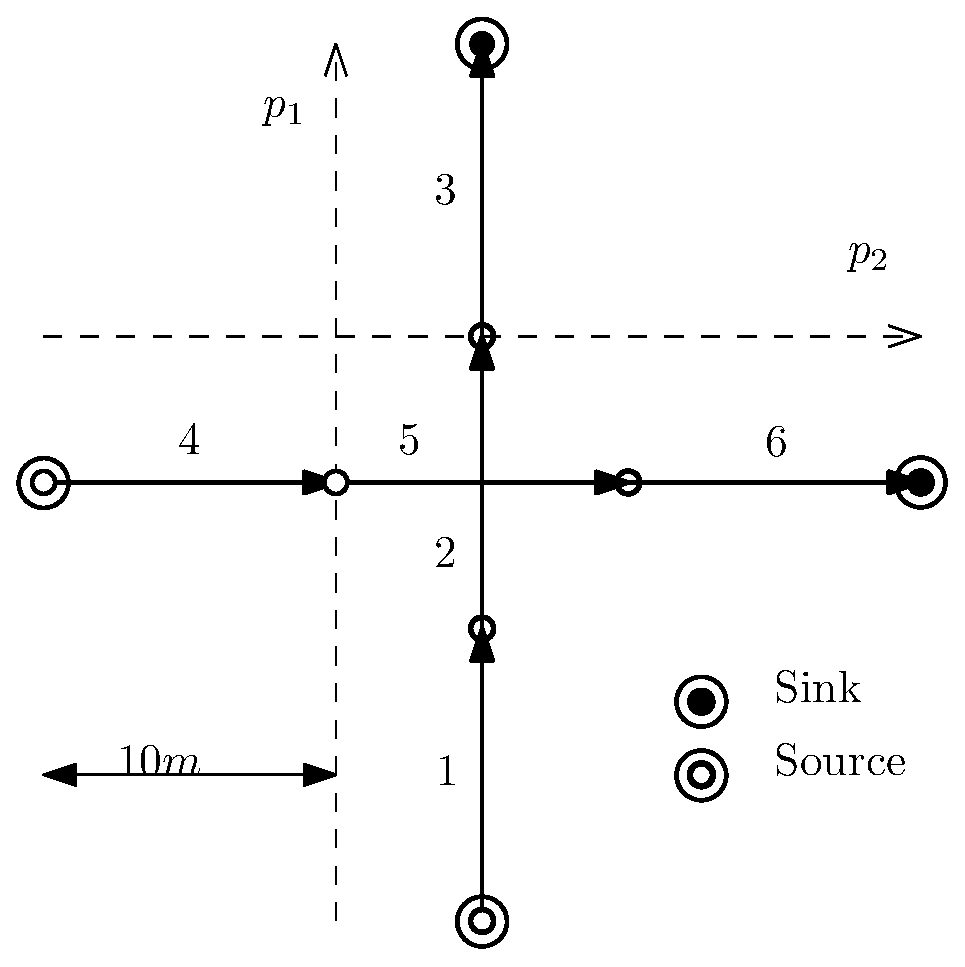
\includegraphics[width=0.9\linewidth]{intersection_topo}
	\caption{Intersection layout with two conflicting routes.}
	\label{fig:layout}
\end{figure}

The intersection controller was implemented based on \cite{Digani2019}. The surrounding lanes are first discretized into segments. The intersection shown in Figure \ref{fig:layout} is divided into six segments, each of length 10 meters. The critical segments are the two that cross in the center. There are two routes defined, one starting on the left and traveling to the right and the other starting at the bottom and traveling up. One AGV takes route 1 and the other takes route 2. If they both travel at maximum speed they will collide in the center.

The dynamic model for each AGV assumes they are able to exactly follow the path, and attempt to reach the target speed for each segment subject to a limited rate of acceleration of $a m/s^2$. 

\begin{figure}[ht]
	\centering
	\includegraphics[width=0.9\linewidth]{SystemSetup3.pdf}
	\caption{Messages exchanged by participants approaching intersection.}
	\label{fig:system_setup}
\end{figure}

The ApproachPlan message sent by the AGV contains a sequence of segments which it intends to traverse, along with its current distance along the first one.  The flow of messages is shown in Figure \ref{fig:system_setup}. The SpeedList sent by the intersection controller contains the optimal speed for every segment in the plan. The speeds can be found with the nonlinear program in Equation \ref{eq:qp_speeds}. 

\subsection{Motor Dynamic and Electrical Model}
The simulated AGV are based on a small payload 100kg total mass, with a maximum speed of 10m/s and peak acceleration of 5m/s$^2$, allowing them to stop safely within 10 metres. The intersection controllers use a constant acceleration model to calculate the time and space deadlines they pass to the AGV. To make the simulation test worthwhile a simulation model with slightly more complexity was used to evaluate the performance.


The brushless DC electric motor used in \cite{Racewicz2018} has suitable properties to propel a 100kg battery powered vehicle. A DC motor can be modelled by the steady state equivalent circuit shown in Figure \ref{fig:dc_circuit} which is well known, for example see \cite{Hughes2008}. 

\begin{figure}[ht]
	\centering
	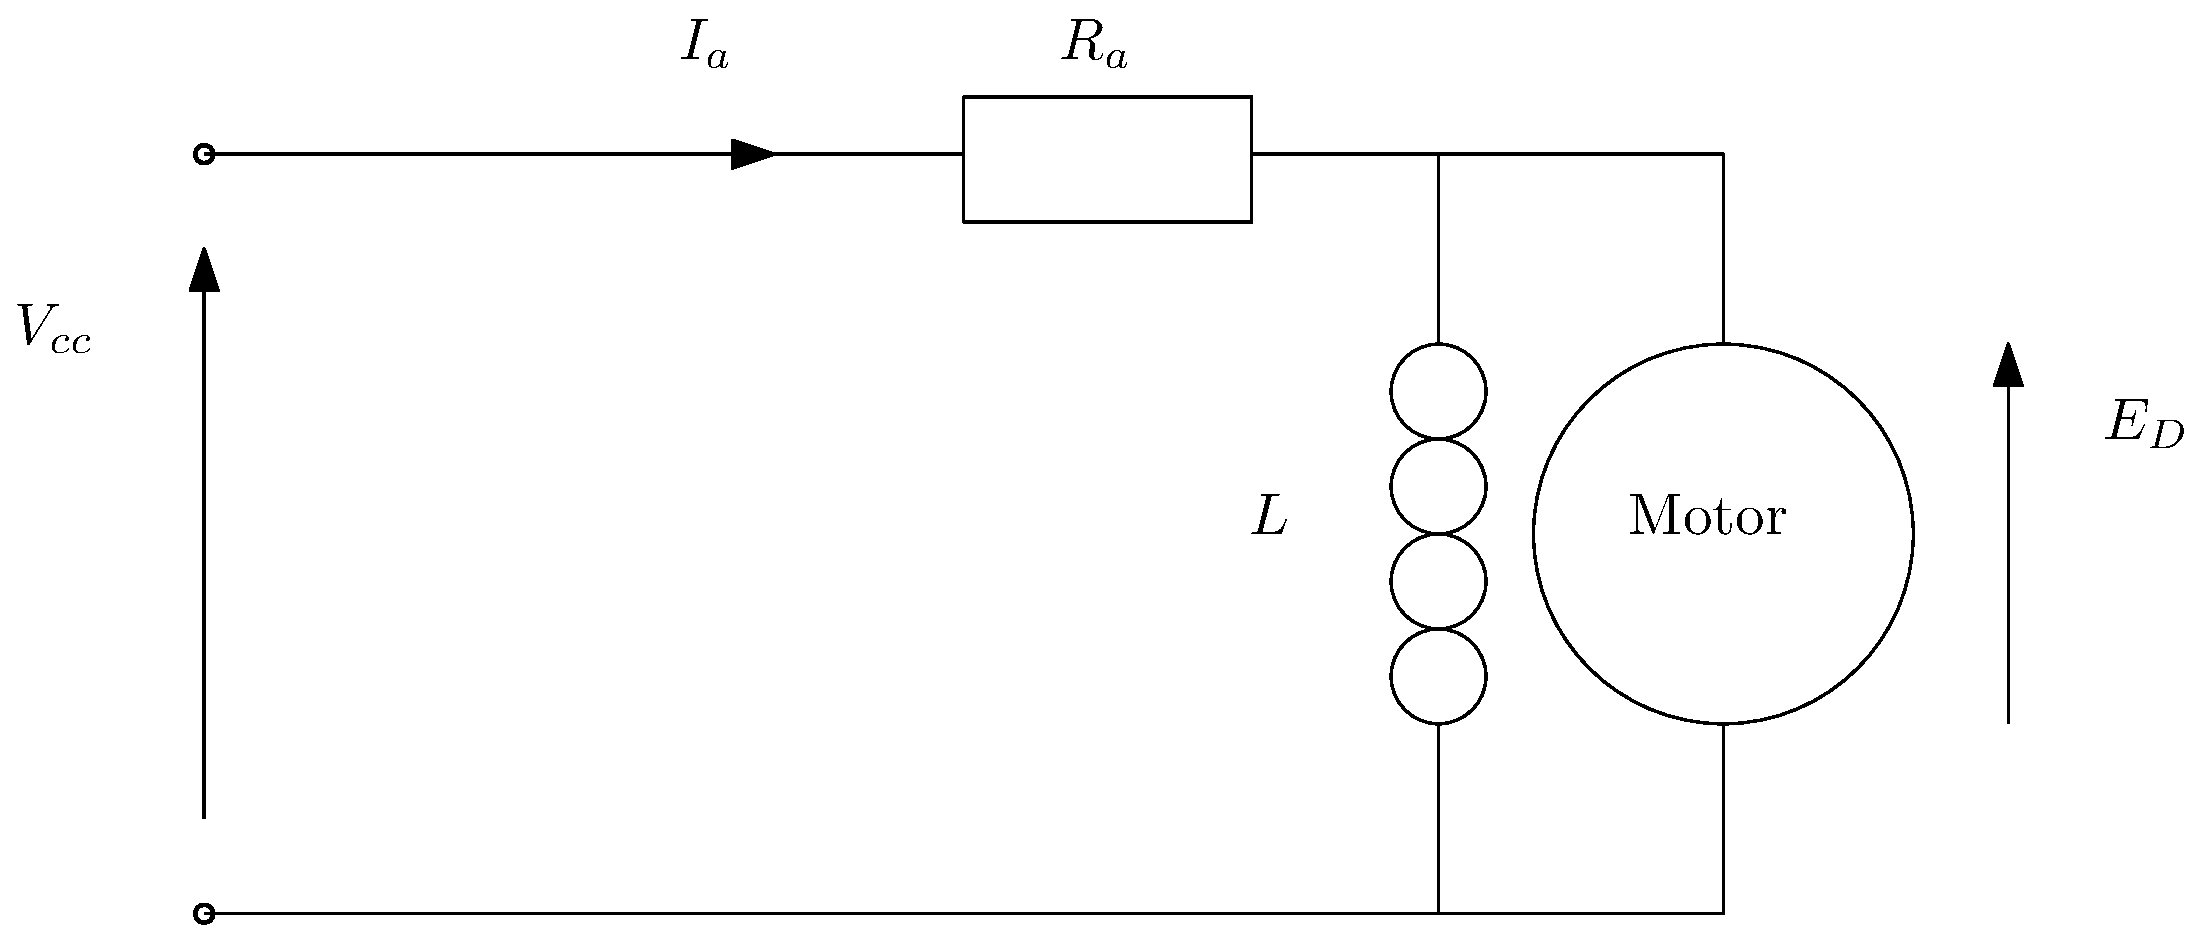
\includegraphics[width=0.9\linewidth]{dc_circuit.eps}
	\caption{Steady state equivalent circuit for a DC motor.}
	\label{fig:dc_circuit}
\end{figure}

This simple circuit leads to the relationship between current and internal resistance given by Equation \ref{eq:steady_state}.
\begin{equation}
	V_{cc} = E_D + I_a R_a
	\label{eq:steady_state}
\end{equation} 
It should be noted that the brushless DC motor is sometimes grouped with AC machines such as the induction motor due to its varying excitation \cite{Sarlioglu2016}. The coils are energised in order to keep the magnetic field at 90 degrees to the field generated by the permanent magnets mounted on the rotor. 

The field strength of the magnets, the number of poles and the number turns of the armature coils can be captured in the motor constant $k_T $ relating torque to armature current.

\begin{equation}
	\tau = k_T I_a
	\label{eq:torque_constant}
\end{equation} 

\begin{equation}
	E_D = \frac{rpm}{k_e}
	\label{eq:emf_constant}
\end{equation} \\

There are numerous loss sources in an electric motor such as winding resistance, flux leakage, eddy currents in the core and so on \cite{Sarlioglu2016}. By using real-world measured mechanical power output and electrical input, an equivalent winding resistance $R_a$ for the simple model can be found. The parameters are shown in Table \ref{tab:motor_params}. 

\begin{table}
	\caption{Motor parameters used in simulation.}
	\label{tab:motor_params} 
	\centering
	\begin{tabular}{ |c|c| }
		\hline
		$k_v$ [rpm/v]& 6 \\ 
		$k_T$ [Nm/A] & 1.53 \\ 
		$P_{mech}$@375rpm [kW] & 3.6 \\ 
		$P_{elec}$@375rpm [kW]& 6.37 \\
		*$R_a$ [Ohms] & 1.0 \\
		\hline
	\end{tabular}
\end{table}

\subsection{Air Resistance}
In addition to the resistive losses in the motor windings losses due to air resistance were also modelled. AGVs  typically operate at low speed <3m/s, hence the unaerodynamic shape of many models. However, the target speed of 10m/s is quite high around 30 miles per hour and drag could become significant. 

The drag coefficient $C_{drag}$=1 for a cuboid shape was used, taken from \cite{Toolbox2004}. The frontal area $A$ of 1m$^2$ is consistent with a box shape for maximum load carrying capacity. The density of air at room temperature is close to 1kg/m$^3$.

\begin{equation}
	F_D = C_{drag} \rho v^2 A
\end{equation} 


\subsection{Arrival Distribution}
%*see Arrival Distribution for Intersection Simulation (Sources!).docx
Previous work in road traffic modelling has used a variety of point distributions to model arrivals. A good summary is given in \cite{Knoop2020} or the chapter on Microsimulation in \cite{Sheffi1985}. 

\subsubsection{Learning from Road Transport Models}
\begin{figure}
	\centering
	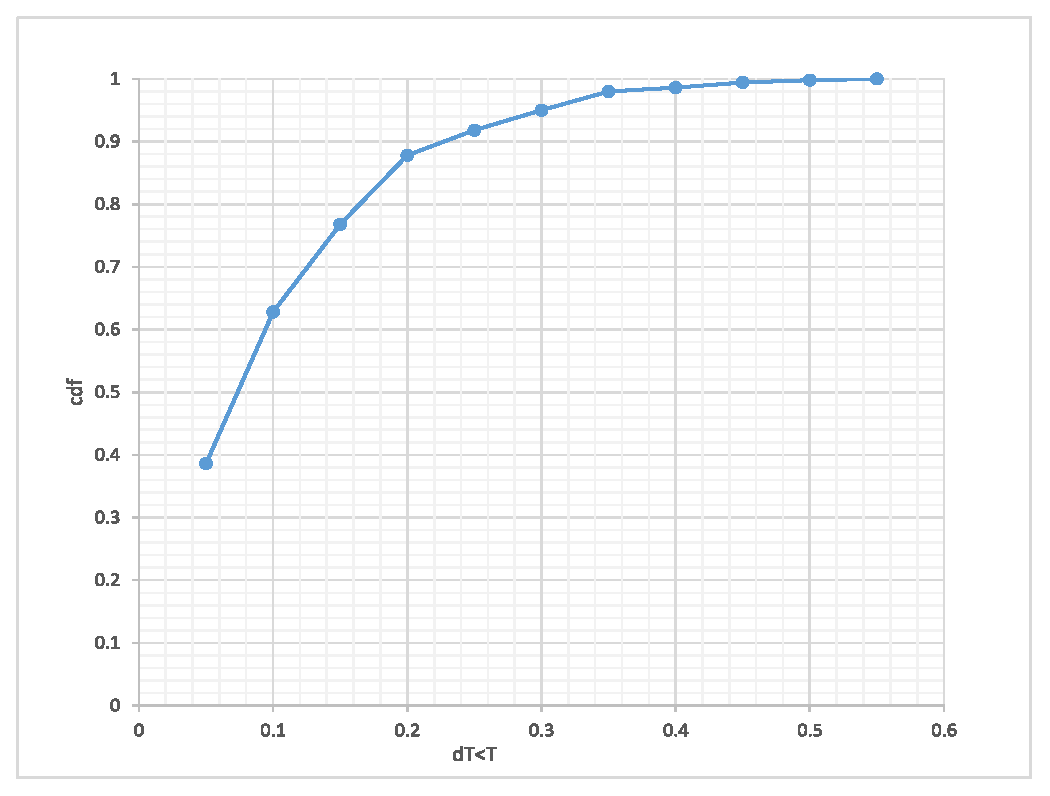
\includegraphics[width=0.9\linewidth]{poisson_cdf.eps}
	\caption{Cumulative Distribution Function of arrivals following a Poisson distribution.}
	\label{fig:poisson_cdf}
\end{figure}
One option is to assume arrivals at a point are completely independent of each other, but occur at an average rate for the time of day which has been measured by inductive loop placed in the road. These assumptions lead to a Poisson distribution such as that shown in Figure \ref{fig:poisson_cdf}. This can be generated computationally by drawing a sequence of numbers from a uniform distribution and applying Equation \ref{eq:poisson_delta} to compute the time delta until the next arrival. To validate the arrivals drawn in this way, we check the log plot of the frequency against time delta is linear and the median is equal to the specified rate as shown in Figure \ref{fig:1_minus_ln_cdf_arr}.   
\begin{figure}
	\centering
	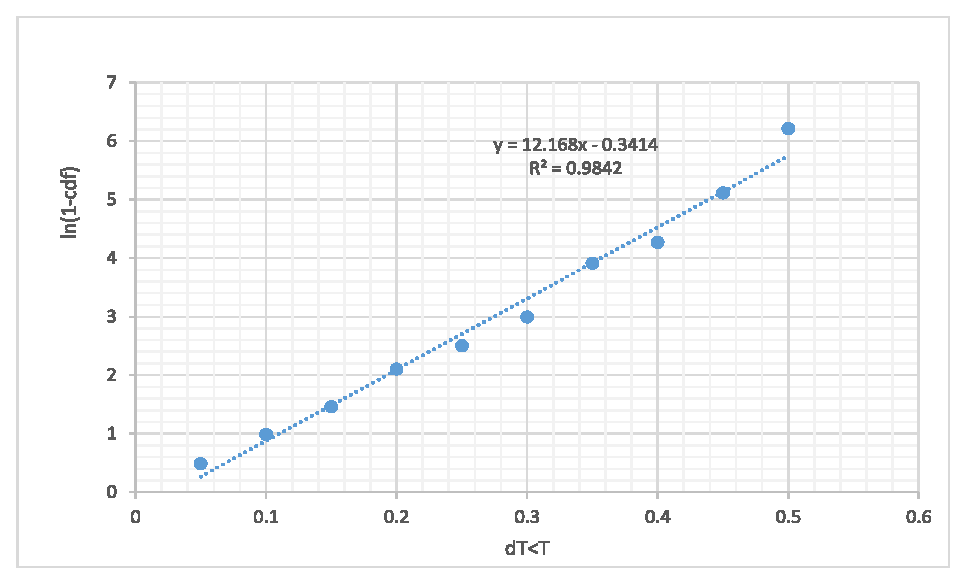
\includegraphics[width=0.9\linewidth]{ln(1-cdf)poisson_arr.eps}
	\caption{Log Cumulative Distribution Function of arrivals with linear fit.}
	\label{fig:1_minus_ln_cdf_arr}
\end{figure}


The assumption that arrivals are independent does not hold if traffic density is high. This is because vehicles slow down to keep a safe distance from the one in front of them. The simplest modification to the poisson distribution to account for this is to discard time deltas which violate the specified safe headway, leading to the shifted exponential distribution. A scatter plot of times from this distribution is shown in Figure \ref{fig:poisson_shifted_scatter}. Now the arrivals will always be realistic in the sense vehicle will not overlap/arrive unsafely but the variance will be smaller. The two parameters the average arrival rate $\lambda$ and the minimum safe headway $\tau$ together control the variance. This is because the median of the distribution must be $\lambda$, so if $1/\tau$ is close to $\lambda$ the variance must be very small.   

\begin{figure}
	\centering
	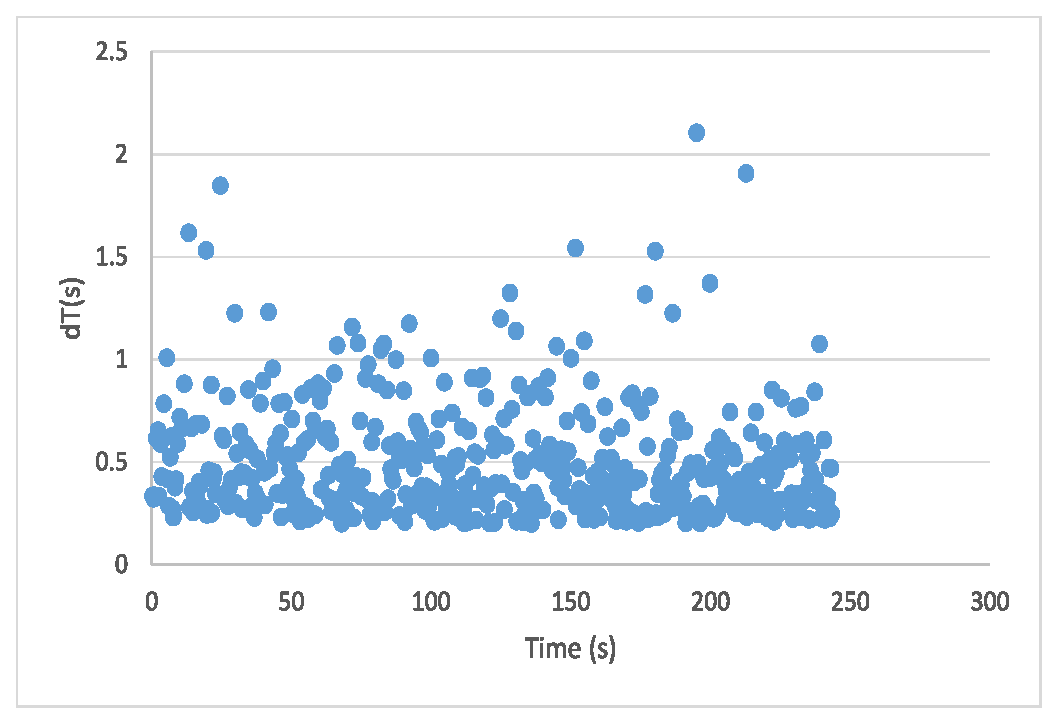
\includegraphics[width=0.9\linewidth]{poisson_shifted_scatter.eps}
	\caption{Scatter plot of 500 arrival time deltas drawn from a shifted exponential distribution with a minimum headway of 0.2 seconds.}
	\label{fig:poisson_shifted_scatter}
\end{figure}
\begin{figure}
	\centering
	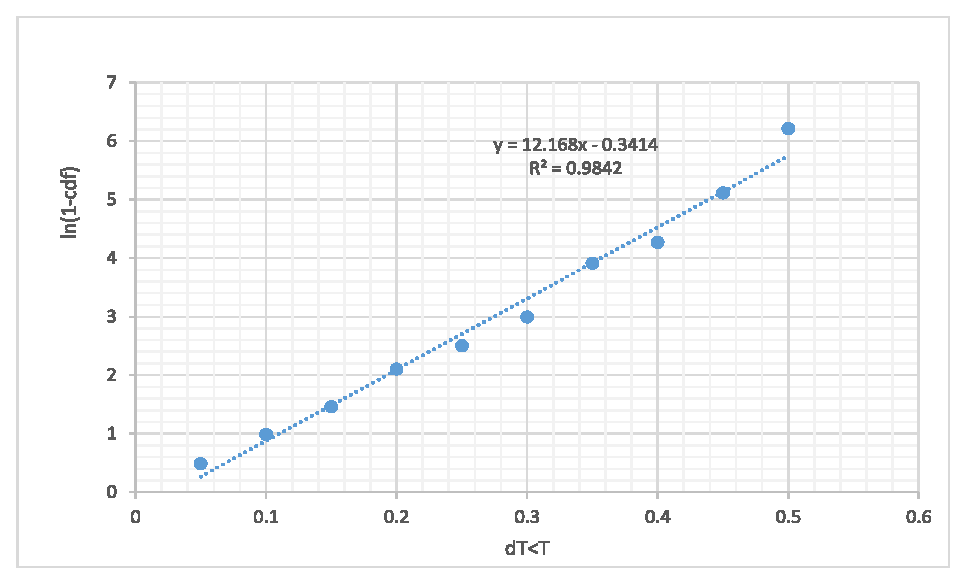
\includegraphics[width=0.9\linewidth]{ln(1-cdf)poisson_arr.eps}
	\caption{Log Cumulative Distribution Function of arrivals with linear fit.}
	\label{fig:1_minus_ln_cdf_arr}
\end{figure}

\subsubsection{Unique Features of AGV Traffic}
The arrival distribution corresponds to the properties of AGV traffic satisfying the following assumptions:
\begin{itemize} 
	\item{More than one AGV is permitted to enter the same link if they are travelling in the same direction.}
	\item{Entry to links in the roadmap is denied if the number already present on the link reaches a fixed capacity}
	\item{Car-following behaviour within the link is governed by the frontal safety system on board each AGV. This provides an outer (warning) zone which, if tripped, the AGV will slow to $w$m/s at $a_w$m/s and an inner zone (emergency)), which if tripped the vehicle will come to a complete stop at $a_e$m/s, where $|a_e|$ > $|a_w|$}
	\item{The capacity of a link is the number of AGVs which would fit without the inner front safety zone of each being tripped by the one in front. This can be calculated for $n$ AGVs each with safety zone length $d_e$ as $n_c = n\dot d_w$}
	\item{Every AGV is informed whether it is able to proceed before it reaches the end of its current link. The AGV will keep slowing down to stop at the end, until it is informed there is space on the next link, at which point it will accelerate to full speed. }
\end{itemize}

According to these assumptions, a suitable model is the shifted exponential, with a minimum headway based on the size of the AGV safety zone. 

\subsubsection{Arrival Variation Based on Approach Lane Occupancy}
Another consideration is how the traffic on the approach lanes should feed back into the arrival times. Based on the counting semaphore for each link assumption, this can be modelled with two queues at the entryway. The lane queue and the busy queue. If the occupancy of the lane is less the $n_c$, new arrivals are added to the lane queue at full speed, in the simulation interval exceeding their point arrival time, at a position they would have reached by the simulation time. If the occupancy of the lane is more than $n_c$ new arrivals are added to the back of the busy queue. At the next time step where $n<n_c$, the AGV at the front of the busy queue is moved onto the lane. The arrival speed is reduced according to acceleration rate $a_W$ based on the time between the arrival and the time step where is can proceed. For longer time periods the new arrival will have zero speed. All arrivals which were not at the front of the busy queue will arrive at the warning speed $v_w$=0.3m/s. 


\subsection{Division of Responsibility Between Intersection and AGV Controllers}
With different signal-free intersection control approaches, the functionality carried out centrally by the fixed-server compared to that by the mobile AGV varies significantly. Of particular interest are the interfaces used by Digani et al \cite{Digani2019} where the intersection provides average speeds for discrete segments, and the one used by Levin and Rey \cite{Levin2017} where the reservation message sent by the intersection contains the arrival time at the conflict point. 

The arrival time at the conflict point is similar to a widely used waypoint interface. As the time is the important quantity for ensuring collisions are avoided this interface seems more sensible. However, on its own it is not sufficient to ensure FIFO behaviour of AGVS approaching in the same lane. Many studies assume an external mechanism for car-following based on local sensors such as the Intelligent Driver Model in \cite{He2020}.  

Without a car-following or platooning approach locally on the AGV, simple methods to manage cross traffic can easily fail to maintain FIFO ordering. This problem is often encountered in traffic simulation with cellular models and there are various techniques to avoid it without generating a trajectory for each vehicle \cite{Carey2014}. 

\cite{Levin2017} and \cite{Digani2019} do not mention any local car following behaviour and seek to avoid all collisions by the centralised application of constraints. This makes it difficult to compare them to a semaphore based intersection controller, unless car following is used in combination with semaphore access control.  

\section{Methods For Zone-Based Intersection}
\subsection{Intersection Controller Objective}
The objective is to minimize $J_T$ the total travel time for all vehicles. It is convenient for exposition to optimize over the inverse of speed of each segment $\phi_k = 1/v_k$. Vehicle $i$ submits a plan containing $m_i$ segments before the conflict and $n_i$ segments in conflict. The control model is based on the average speed of each approaching AGV over each segment. This is to simplify the description of the intersection controller, and assist analysis. More sophisticated motion models could take the place of  Equation \ref{eq:omega_min} and  Equation \ref{eq:omega_max} to create a similar type of problem with a convex travel time objective and non-convex constraints.   
The parameters for one vehicle can be collected in the vector $\bm{\phi}_i$ as shown in Equation \ref{eq:phi_i}
\begin{equation}
	\bm{\phi}_i =  [\phi_{1}, ..., \phi_{(m_i + n_i)}]^T \\
	\label{eq:phi_i}
\end{equation}
The parameters for $p$ vehicles each traversing $(m_i + n_i)$ segments are assembled into a vector as in Equation \ref{eq:parameters}
\begin{equation}
	\bm{\phi} = [\bm{\phi_{1}}^T, ..., \bm{\phi}_{p}^T]^T \\
	\label{eq:parameters}
\end{equation}
Similarly, the length of each segment in plan $i$ can be arranged into a vector 
\begin{equation}
	\bm{d}_i = [d_{1}, ..., d_{(m_i + n_i)}]^T \\
	\label{eq:d_i}
\end{equation}
and collected  for $p$ vehicles into a vector as in Equation \ref{eq:d}.
\begin{equation}
	\bm{d} = [\bm{d_{1}}^T, ..., \bm{d}_{p}^T]^T \\
	\label{eq:d}
\end{equation}
This leads to the minimum travel time objective in Equation \ref{eq:qp_speeds}. 
\begin{equation}
	\begin{array}{c}
		\min \limits_{\bm{\phi}} \bm{J_T} = \bm{d}^T \bm{\phi} \\
		\textrm{subject to}\\
		\bm{\phi}_{max} > \bm{\phi} > \bm{\phi}_{min} \\
		\bm{\phi}^T\bm{H}_{i,j}\bm{\phi} > \bm{0} \quad \forall i,j \in [1,p] \quad \textrm{with } j>i \\
	\end{array}
	\label{eq:qp_speeds}
\end{equation}

The condition $j>i$ in Equation \ref{eq:qp_speeds} indicates that the number of constraints varies with the number of vehicles $p$ as $\frac{p(p-1)}{2}$. This corresponds to one constraint between each pair of approaching AGVs.

\subsection{Intersection Controller Timing Constraints}
By definition, each intersection has a single conflict zone, the union of all segments which intersect there. This makes it possible to express the constraint that vehicles do not collide in terms of time. Vehicle $i$ arrives at the first conflicted segment $\omega_i^{min}$ and departs from the last at $\omega_i^{max}$. The following three subsections set out three alternative ways of expressing the collision avoidance constraints which have been evaluated. 
The arrival time is given by Equation \ref{eq:omega_min}. Considering average speeds, the departure time $\omega_i^{max}$ is also linear, this is given by Equation \ref{eq:omega_max}. 
\begin{equation}
	\omega_i^{min}  = \sum_{k=1}^{m_i} \bm{d}_i [k] \bm{\phi}_i [k] = \bm{e}^T \bm{\phi}_i
	\label{eq:omega_min}
\end{equation}
where %$\bm{e}[k] = \bm{d}_i[k] \forall k <m_i, otherwise 0$
\begin{equation}
	\bm{e}[k] = \left\{
	\begin{array}{cc}
		\bm{d_i}[k] & \forall k <m_i \\
		0 & \textrm{otherwise} \\
	\end{array}
	\right.
\end{equation}  and $m_i$ is the number of segments on the path of vehicle $i$ before arrival at the conflicted segment. 
\begin{equation}
	\omega_i^{max}  = \omega_i^{min} + \sum_{i=1}^{n_i} \bm{d}_i [k] \bm{\phi}_i [k] = \bm{f}^T \bm{\phi}_i
	\label{eq:omega_max}
\end{equation}
where 
\begin{equation}
	\bm{f}[k] = \left\{
	\begin{array}{cc}
		\bm{d_i}[k] & \forall k <m_i+n_i \\
		0 & \textrm{otherwise} 
	\end{array}
	\right.
\end{equation}
and $n_i$ is the number of segments on the path of vehicle $i$ which are conflicted. Note that Equations \ref{eq:omega_min} and \ref{eq:omega_max} only depend on the $\bm{\phi}_i$ of vehicle $i$. 



\subsubsection{Linear FIFO Constraints}
\label{sec:fifo_constraints}
If the order in which the AGV cross the conflict zone is fixed to be First-In-First-Out, the timing constraint is linear. For a pair where the leader enters the conflict at $t_i$ and takes $\Delta t_i$ seconds to cross at maximum speed the condition for entry time of the follower $t_{i+1}$ given by Equation \ref{eq:entry_time}.

\begin{equation}
	-t_{i} + t_{i+1}	\leq	\Delta t_i
	\label{eq:entry_time} 
\end{equation} 

There is one constraint between each adjacent pair so $p-1$ constraints total for $p$ vehicles. These can be expressed in the form $\bm{A}_{ub}\phi \leq \bm{b}_{ub}$ as in Equation \ref{eq:fifo}. This is correct for two AGV arranged in distance order, each traversing one approach and one conflict segment. 



\begin{equation}
	\left[ 
	\begin{array}{ccccc}
		-d_1 & d_2 & \bm{0}\\
		\vdots & \ddots & \vdots \\
		\bm{0} & -d_{p-1} & d_p\
	\end{array} \right]
	\left[
	\begin{array}{c}
		\phi_1 \\ \vdots \\ \phi_p
	\end{array} \right]
	\leq
	\left[ 
	\begin{array}{c}
		\Delta t_1 \\
		\vdots \\
		\Delta t_{p-1}
	\end{array} \right]
	\label{eq:fifo}
\end{equation}

The timing constraint between each pair of vehicles can be expressed with a modulus operator as in Equation\ref{eq:timing}.
\begin{equation}
	|\alpha_i - \alpha_j| > \beta_i + \beta_j
	\label{eq:timing}
\end{equation}

Here 
\begin{equation}
	\alpha_i  = \omega_i^{max} + \omega_i^{min}
	\label{eq:alpha}
\end{equation}
represents the midpoint of the time vehicle $i$ occupies the conflicted segment and
\begin{equation}
	\beta_i  = \omega_i^{max} - \omega_i^{min}
	\label{eq:beta}
\end{equation}
represents the range of the time either side of the midpoint, both scaled by a factor of two. 


In matrix form
\begin{equation}
	\alpha_i  = \bm{f}^T \bm{\phi}_i + \bm{e}^T \bm{\phi}_i = \bm{1}_i^T\bm{A}{\phi}_i
	\label{eq:alpha_m}
\end{equation}
with $\bm{A} = diag(\bm{f} + \bm{e})$
\begin{equation}
	\beta_i  = \bm{f}^T \bm{\phi}_i - \bm{e}^T \bm{\phi}_i =  \bm{1}_i^T\bm{B}{\phi}_i
	\label{eq:beta_m}
\end{equation}
with $\bm{B} = diag(\bm{f} - \bm{e})$

The resulting linear program (with parameters $\in\mathbb{R}$) has $p-1$ constraints as each AGV is only constrained by the preceding one.

\subsubsection{Quadratic Constraints}
\label{sec:quad_constraints}
Another way to treat the modulus operator in Equation \ref{eq:timing}, without forcing any particular arrival order is to square both sides as to give the expression in Equation \ref{eq:expanded}. 
\begin{equation}
	\alpha_i^2 - \alpha_j^2 - 2 \alpha_i\alpha_j - (\beta_i^2 + \beta_j^2 +2 \beta_i \beta_j) > 0
	\label{eq:expanded}
\end{equation}
Collecting terms by subscript gives
\begin{equation}
	(\alpha_i^2 - \beta_i^2) - (\alpha_j^2 + \beta_j^2) - 2(\alpha_i\alpha_j + \beta_i \beta_j) > 0
	\label{eq:collected}
\end{equation}

The matrix $\bm{\Lambda}_ij$ captures the constraints between a pair of vehicles and always contains four sub-matrices as shown in in Equation \ref{eq:lambda}. It is compatible with $\bm{\phi}_{i,j} = [\bm{\phi}_i^T, \bm{\phi}_j^T]^T$, containing only the relevant speeds for vehicles $i$ and $j$. 
\begin{equation}
	\bm{\Lambda}_{ij} =\left[
	\begin{array}{cc}
		\bm{\Lambda}_{ij}^{ii} & \bm{\Lambda}_{ij}^{ij} \\
		\bm{\Lambda}_{ij}^{ji} & \bm{\Lambda}_{ij}^{jj} \\
	\end{array}
	\right]
	\label{eq:lambda}
\end{equation}
Expanding 
\begin{multline}
	\left[\bm{\phi}_i^T, \bm{\phi}_j^T\right]
	\left[\begin{array}{cc}
		\bm{\Lambda}_{ij}^{ii} & \bm{\Lambda}_{ij}^{ij} \\
		\bm{\Lambda}_{ij}^{ji} & \bm{\Lambda}_{ij}^{jj} \\
	\end{array}\right]
	\left[\begin{array}{c}
		\bm{\phi}_i\\
		\bm{\phi}_j \end{array} \right] \\
	= \bm{\phi}_{i}^T \bm{\Lambda}_{ij}^{ii} \bm{\phi}_{i} + \bm{\phi}_{j}^T \bm{\Lambda}_{ij}^{jj} \bm{\phi}_{j} + \bm{\phi}_{i}^T \bm{\Lambda}_{ij}^{ij} \bm{\phi}_{j} + \bm{\phi}_{j}^T \bm{\Lambda}_{ij}^{ji} \bm{\phi}_{i}
\end{multline}
makes it possible to compare terms with the scalar expression in Equation \ref{eq:collected}. This leads to the following expressions for the submatrices in $\Lambda$ in terms of $\alpha_i = \bm{1}_T\bm{A}_i\bm{\phi}_i$ and $\beta_i = \bm{1}_T\bm{B}_i\bm{\phi}_i$ 
\begin{equation}
	\bm{\Lambda}_{ij}^{ii} = (\bm{A}_i - \bm{B}_i)\bm{1}_i\bm{1}_i^T(\bm{A}_i - \bm{B}_i) 
	\label{eq:ii}
\end{equation}
\begin{equation}
	\bm{\Lambda}_{ij}^{jj} = -(\bm{A}_j + \bm{B}_j)\bm{1}_j\bm{1}_j^T(\bm{A}_J + \bm{B}_j) 
	\label{eq:jj}
\end{equation}
\begin{equation}
	\bm{\Lambda}_{ij}^{ij} + \bm{\Lambda}_{ij}^{ij T} = -2(\bm{A}_j + \bm{B}_j)\bm{1}_j\bm{1}_i^T(\bm{A}_i + \bm{B}_i) 
	\label{eq:ij}
\end{equation}

For more than two vehicles this can be arranged into a block diagonal matrix $\bm{H}_{ij}$ which is compatible with the input parameters, but still only represents the constraints between a pair. 

Expressed in this way it is clear the constraints are quadratic and it is trivial to differentiate twice to find the Hessian is the stack of constraint matrices $[\bm{H}_{ij}, \hdots]$. The objective is certainly convex as it is linear but the constraints may not be. If the Hessian of the constraints is positive semi-definite then they are convex and interior point methods will either find the global optimum or prove that there is no feasible solution \cite{Boyd2004}. The Hessian depends on the parameters of the roadmap, the number of approaching vehicles and their distance from the conflict. 

\subsubsection{Mixed Integer Constraints}
\label{sec:milp_constraints}
A third way of treating the timing constraint in Equation \ref{eq:timing}, also without forcing any particular arrival order involves splitting each constraint into two based on the sign of $(\alpha_i-\alpha_j)$ as shown in equation \ref{eq:or_cons}. Again, this is expressed in terms of the midpoint $\alpha_i$, $\alpha_j$ and extent $\beta_i$,$\beta_j$ of the time when vehicle $i$ and vehicle $j$ occupy the segment on their own path which passes through the conflict point,
\begin{equation}
	\begin{array}{cc}
		\alpha_i - \alpha_j > \beta_i + \beta_j &\textrm{if  }\alpha_i >\alpha_j  \\
		\alpha_i - \alpha_j < -(\beta_i + \beta_j) & \textrm{otherwise}\\
		\textrm{where } \alpha_i, \alpha_j, \beta_i, \beta_j >0
	\end{array}
	\label{eq:or_cons}
\end{equation}
In order to apply these OR constraints, an additional integer parameter $b_k$ can be introduced for each pair of AGV, along with an arbitrary large number $M$ as shown in Equation \ref{eq:big_m_cons}. 
\begin{equation}
	\begin{array}{cc}
		\alpha_i - \alpha_j + b_{i,j}M > \beta_i + \beta_j \\
		\alpha_i - \alpha_j - (1-b_{i,j})M < -(\beta_i + \beta_j) \\
		\textrm{where } b_{i,j}\in[0,1] \\
		M>>\alpha_i, \alpha_j, \beta_i, \beta_j
	\end{array}
	\label{eq:big_m_cons}
\end{equation}
Now the problem is combinatorial rather than convex and appropriate methods must be used. These may be based on exhaustive search such as Branch-and-Bound, or solving a sequence of convex relaxations of the original problem \cite{Murray2010}. Combinatorial problems quickly become intractable for large numbers of variables, but in this case the underlying problem of arrival order is combinatorial, so exhaustive methods are needed to find the global minimum. 

It is possible to further assume every AGV travels at maximum speed once it reaches the conflict, simplifying equation Equations \ref{eq:alpha} and \ref{eq:beta} with a constant $p_i = g_i \phi_{min}$. 
\begin{equation}
	\alpha_i = 2\omega_i^{min} + p_i
\end{equation}
\begin{equation}
	\beta_i = p_i
\end{equation}
where $g_i$ is the length of the conflicted segments in the plan of vehicle $i$. In this case Equation \ref{eq:big_m_cons} can be restated 
\begin{equation}
	\begin{array}{cc}
		\omega_i^{min} - \omega_j^{min} + b_{i,j}M > p_j \\
		\omega_i^{min} - \omega_j^{min}  - (1-b_{i,j})M < -p_i \\
		\textrm{where } b_{i,j}\in[0,1] \\
	\end{array}
	\label{eq:minlp}
\end{equation}

\section{Methods For Conflict Point Intersection}
For a intersection between roads with multiple lanes, it makes sense to plot the centreline of each lane, and the arc of each turning motion between lanes. Any point where two of these arcs cross is called a conflict point. By controlling arrival time at a conflict point, collisions can be avoided, while vehicles that do not pass the same conflict point can both proceed \cite{Levin2017}.

\begin{figure}[ht]
	\centering
	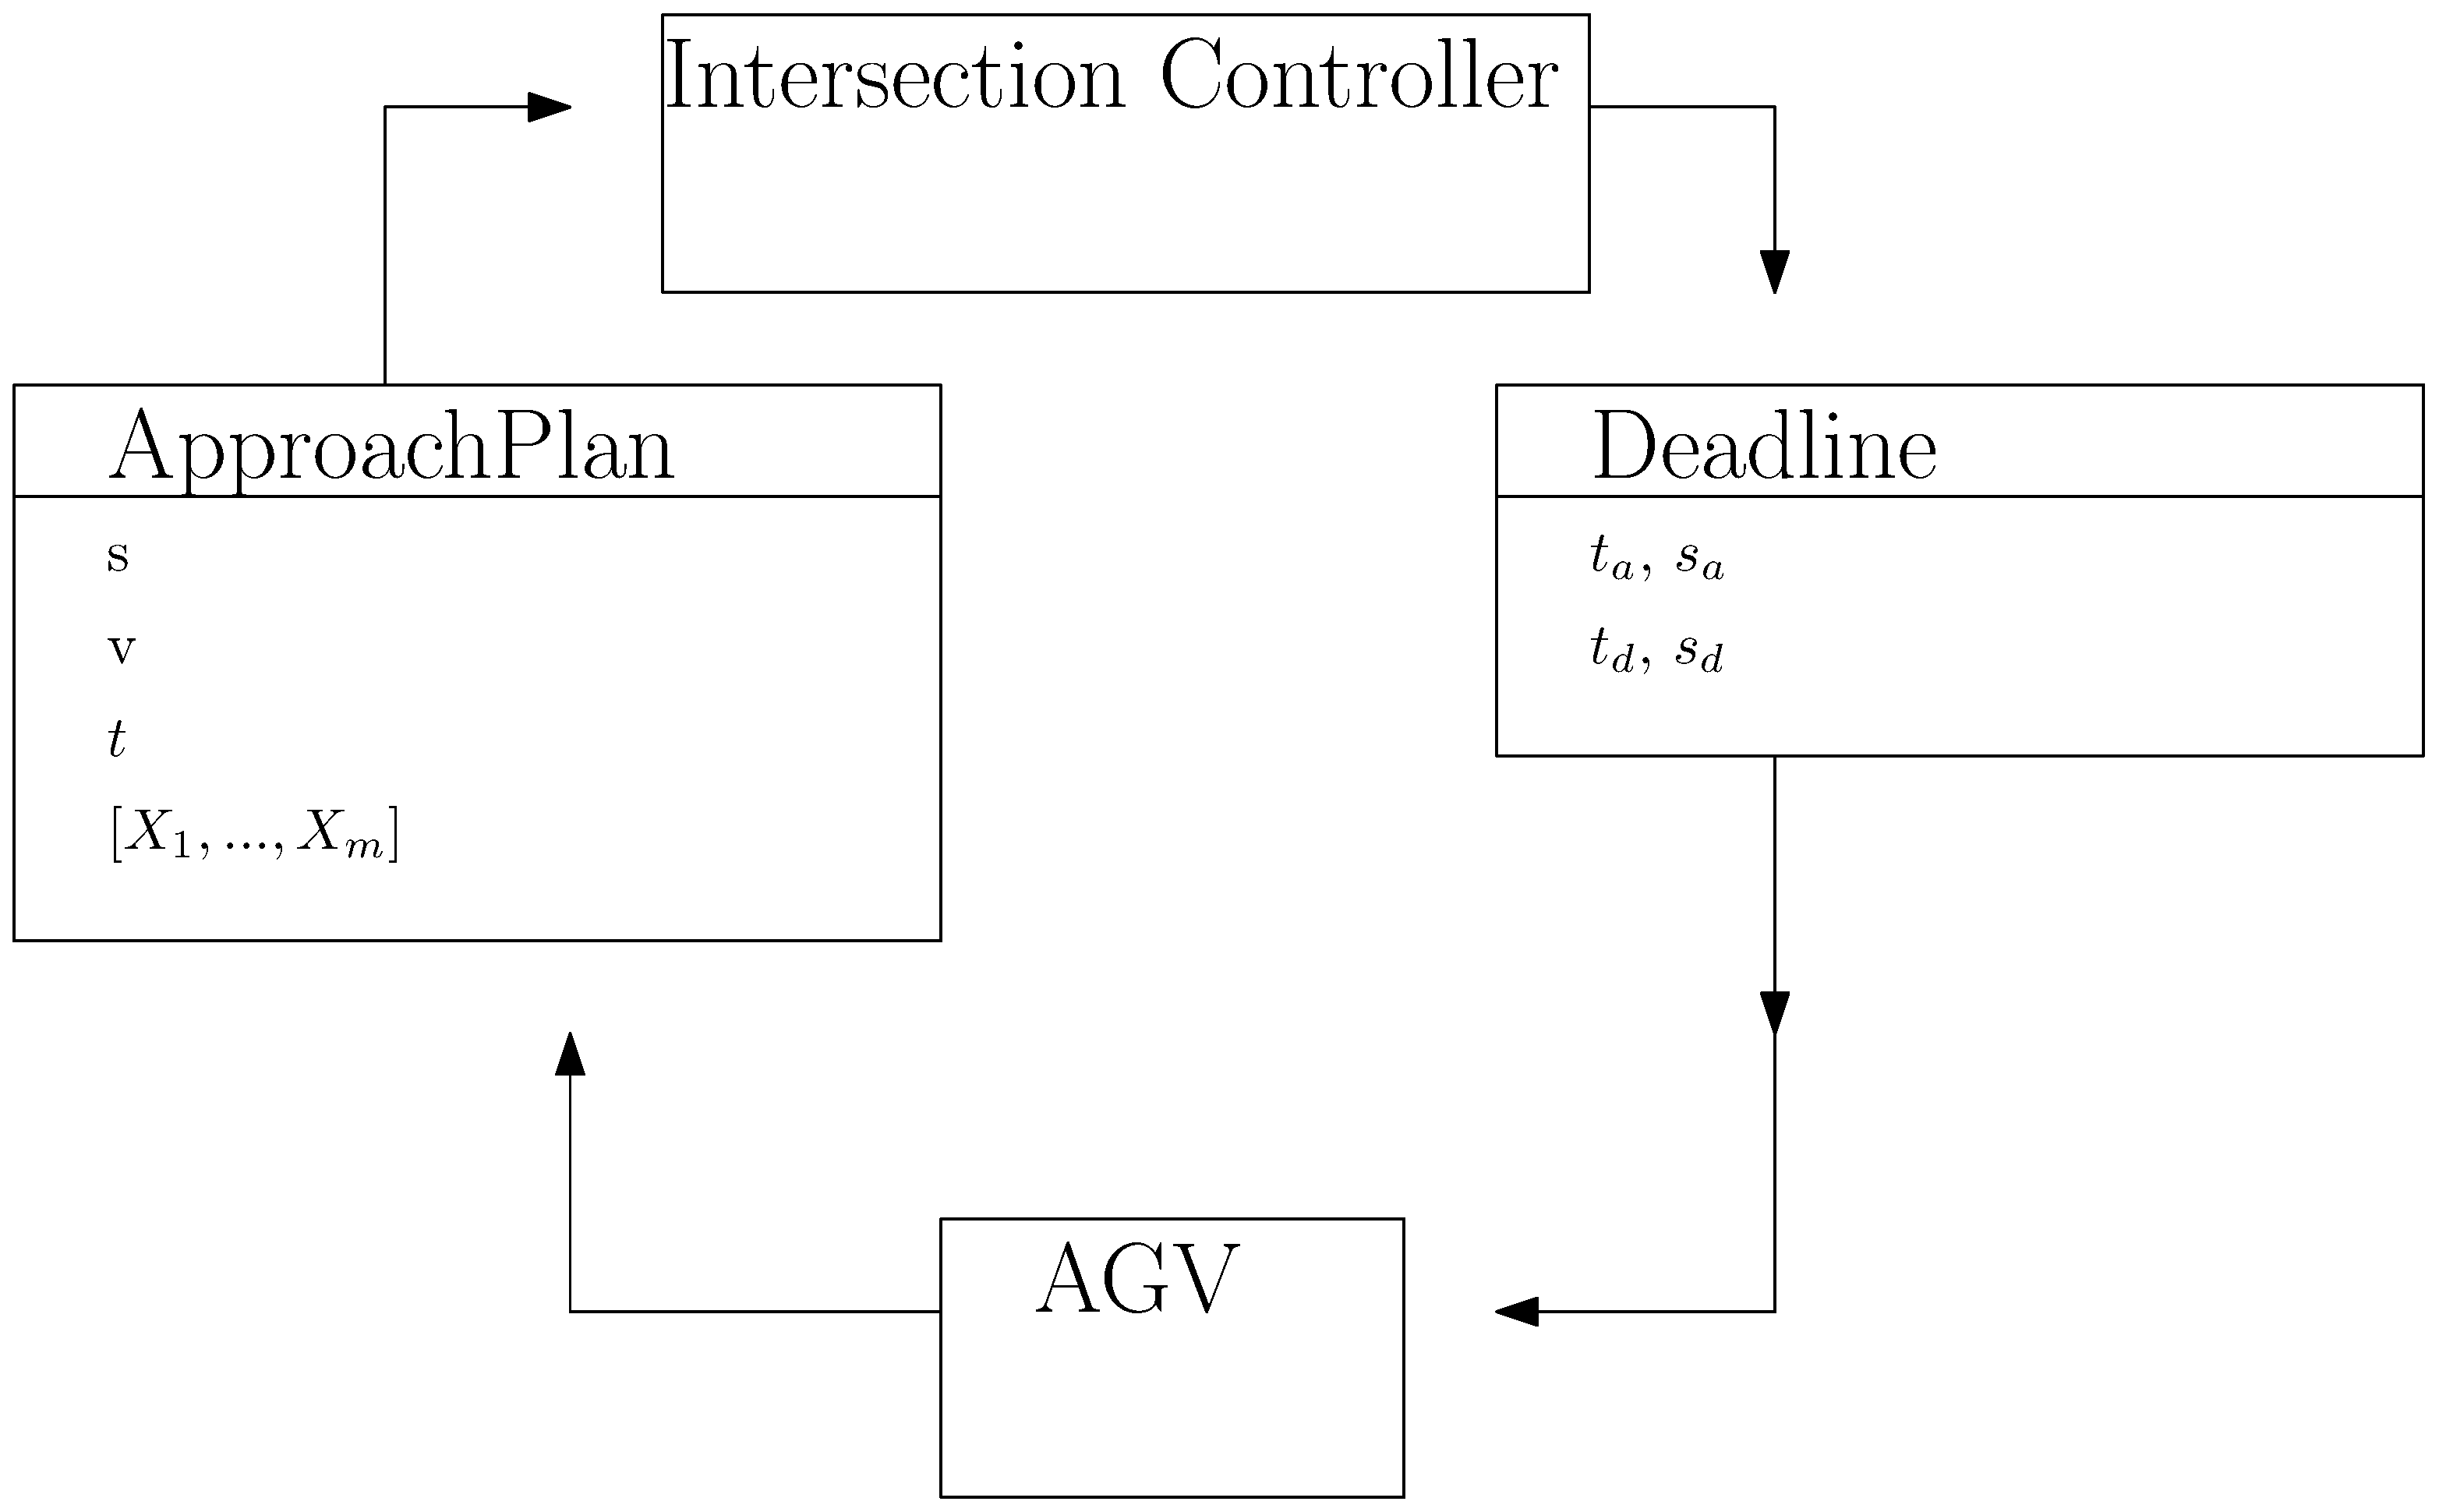
\includegraphics[width=0.9\linewidth]{plan_deadline_interface.eps}
	\caption{Key messages of the ``Plan/Deadline'' interface governing access to a conflict point intersection.}
	\label{fig:plan_deadline_interface}
\end{figure}

A controller based on a common heuristic for controlling access to a shared resource, the binary semaphore, is included for comparison with the optimal methods.  Similar approaches are widespread in AGV control \cite{Duinkerken1999} and \cite{Lee2019}.


\subsection{Semaphore Approach}
To implement the ``plan/deadline'' interface, a binary semaphore for each conflict point was needed. The semaphore controller does not compute the entry and exit times of the conflict as it has is no model of the vehicle dynamics. It simply raises the semaphore, sending a ``full speed ahead'' message to the closest AGV to the intersection and a position deadline to all others.

For this reason the deadline message contains the position at which the AGV must stop, without any timing. The AGV must stop at the given position until it receives a `proceed' message form the intersection controller.

\section{Performance Comparison}
Both conflict point representation and the zone representation are identical if the intersection has exactly one conflict. On this basis the semaphore approach and two versions of minimum crossing time optimal control, one with FIFO linear constraints and the other with quadratic constraints were compared on a simulated intersection comprising two lanes which cross in the middle. The approach distance is fixed at 15 metres.

The controllers will be tested with traffic levels and control latencies intended to bound the likely values of these parameters, shown in Table \ref{tab:test_params}.

\begin{table}
	\caption{Parameters bounds used to generate test scenarios.}
	\label{tab:test_params} 
	\centering
	\begin{tabular}{ |c|c|c| }
		\hline
		Parameter & High Bound & Low Bound \\
		$T_C$ [s]& 0.5 & 0.1 \\ 
		$\frac{1}{\lambda}=\Delta T_a$ [s]& 10 & 2 \\ 	
		\hline
	\end{tabular}
\end{table}

\begin{table}
	\begin{tabular}{|c|c|c|c|}
		\hline
		& $\lambda_1$ & $\lambda_2$ & $f$ \\
		\hline
		HLHT & 0.5 & 0.5 & 2 \\
		HLMT & 0.1 & 0.5 & 2 \\
		HLLT & 0.1 & 0.1 & 2 \\
		LLHT & 0.5 & 0.5 & 10 \\
		LLMT & 0.1 & 0.5 & 10 \\
		LLLT & 0.1 & 0.1 & 10 \\
		\hline
	\end{tabular}
	\label{tab:params}
	\caption{Parameters for test scenarios. All units s$^-1$. Each scenario is identified with the first two characters relating to the latency between periodic messages from the intersection controller where High Latency is 500ms and  Low Latency is 100ms and the second two relating to the arrival rate, where High Traffic has $\lambda$=10 arrivals per second on both approaches, Low Traffic has $\lambda$=2 arrivals per second on both, and Mixed Traffic has one lane with $\lambda_1$=10 and the other with $\lambda_2$=2. For example High Latency, High Traffic becomes HLHT.}
\end{table}

\section{Simulation Results}

\begin{figure}[ht]
	\centering
	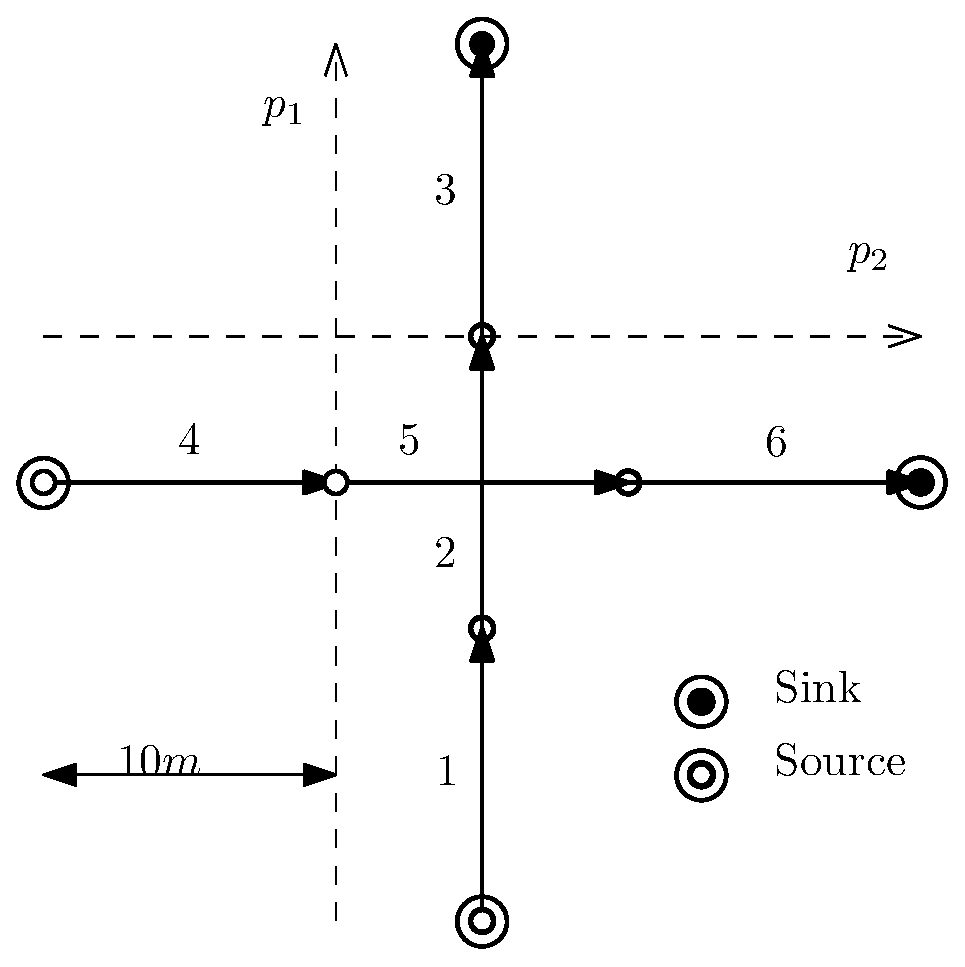
\includegraphics[width=0.9\linewidth]{intersection_topo}
	\caption{Intersection layout with two conflicting routes.}
	\label{fig:intersection_topo}
\end{figure}

The different approaches to intersection control were evaluated on a simulation of a simple intersection, comprised of two 30m lanes which cross in the middle as shown in Figure \ref{fig:intersection_topo}. There are two entrances to the map, one at the start of each lane. By varying the arrival rate $\lambda$ and the update frequency $f$, six scenarios were created with the parameters shown in Table \ref{tab:params}.
\begin{table}
	\begin{tabular}{|c|c|c|c|}
		\hline
		& $\lambda_1$ & $\lambda_2$ & $f$ \\
		\hline
		HLHT & 0.5 & 0.5 & 2 \\
		HLMT & 0.1 & 0.5 & 2 \\
		HLLT & 0.1 & 0.1 & 2 \\
		LLHT & 0.5 & 0.5 & 10 \\
		LLMT & 0.1 & 0.5 & 10 \\
		LLLT & 0.1 & 0.1 & 10 \\
		\hline
	\end{tabular}
	\label{tab:params}
	\caption{Parameters for test scenarios. All units s$^-1$. Each scenario is identified with the first two characters relating to the latency between periodic messages from the intersection controller where High Latency is 500ms and  Low Latency is 100ms and the second two relating to the arrival rate, where High Traffic has $\lambda$=10 arrivals per second on both approaches, Low Traffic has $\lambda$=2 arrivals per second on both, and Mixed Traffic has one lane with $\lambda_1$=10 and the other with $\lambda_2$=2. For example High Latency, High Traffic becomes HLHT}
\end{table}

\subsection{Trajectory Comparison with Fixed Arrival Pattern, 30 Second Run}
\label{sec:fixed_arrival_pattern}
\begin{figure}
	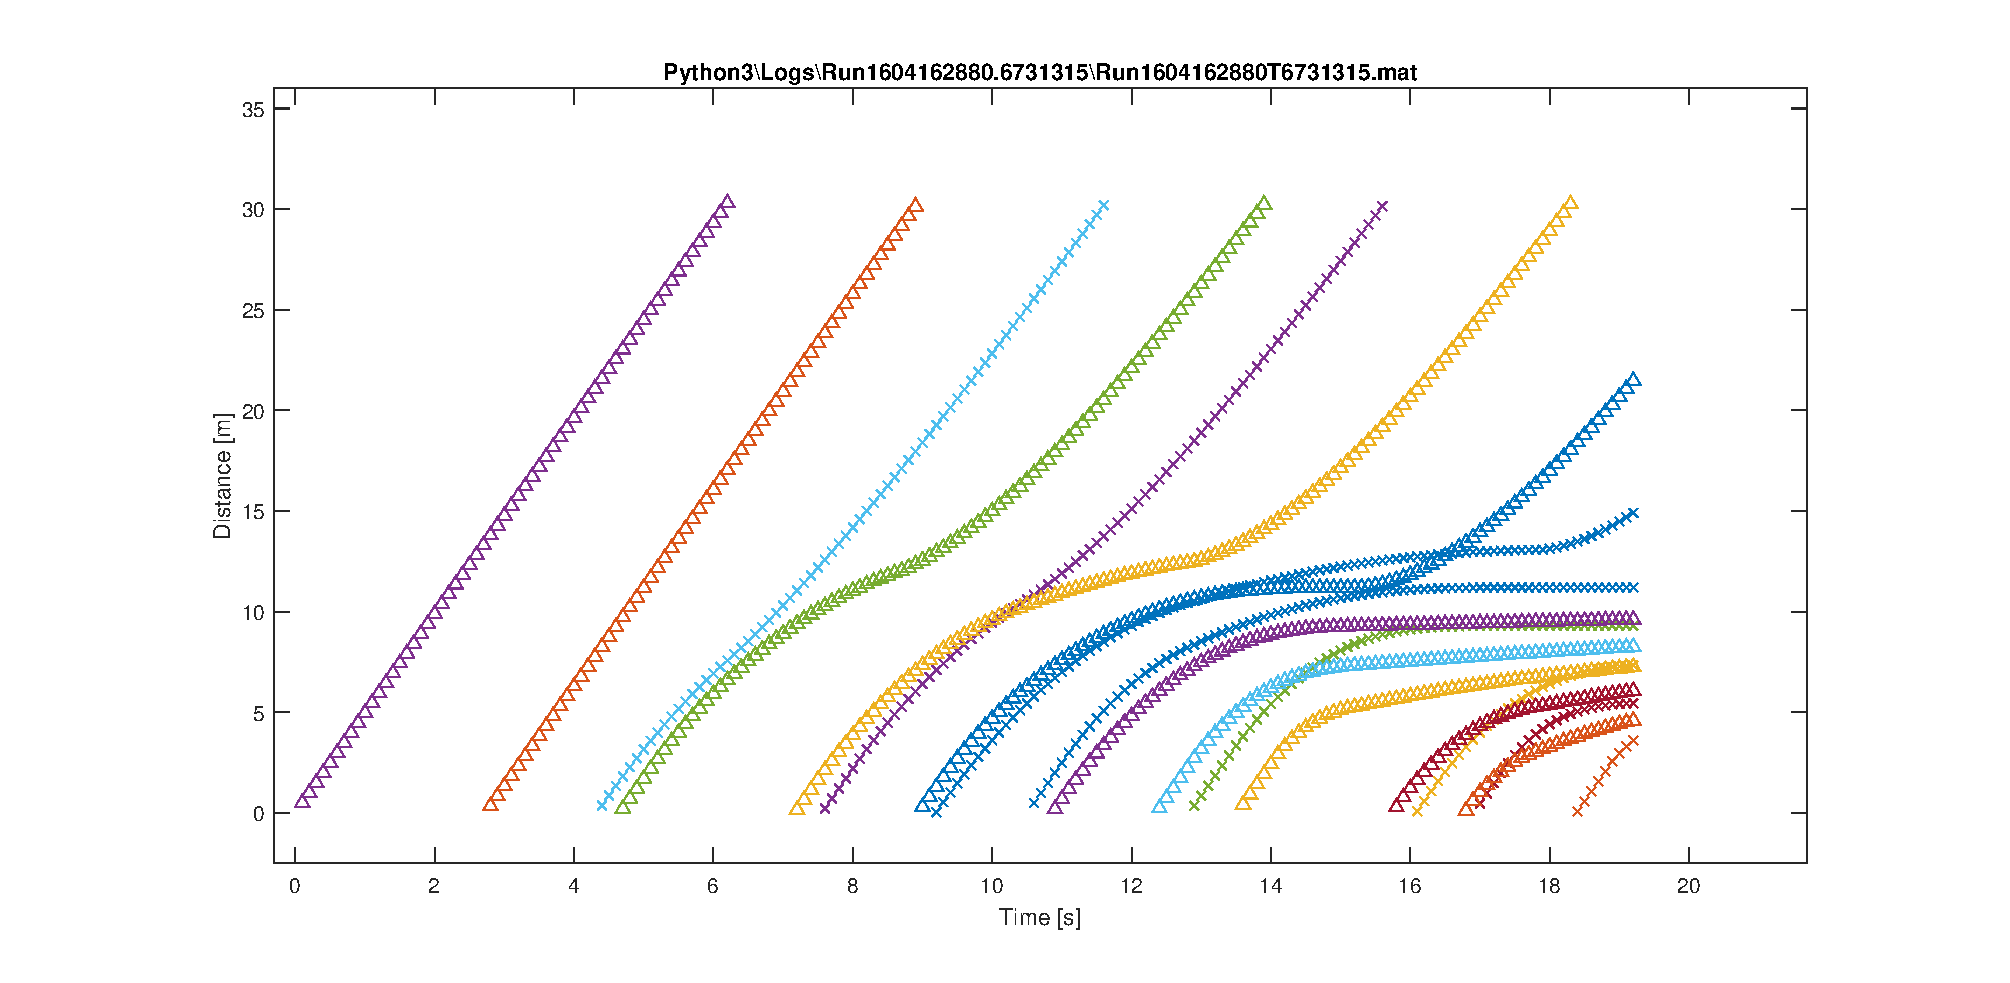
\includegraphics[width=1.0\linewidth]{SemaphoreTracesT6731315.eps}
	\caption{Position time series for the semaphore heuristic controller in scenario 1.}
	\label{fig:semaphore_st}       % Give a unique label
\end{figure}
The distance-time plot for the semaphore controller is shown in Figure \ref{fig:semaphore_st}. The distance axis is measured from the start of the submitted plan for the AGV. All plans start 15 metres from the conflict point on both lanes. AGV travelling in the x-direction are shown with 'x' markers, while those travelling in the y-direction are shown with triangle markers. The simulation did not proceed beyond 20 seconds because of a collision with a new arrival. 

\begin{figure}
	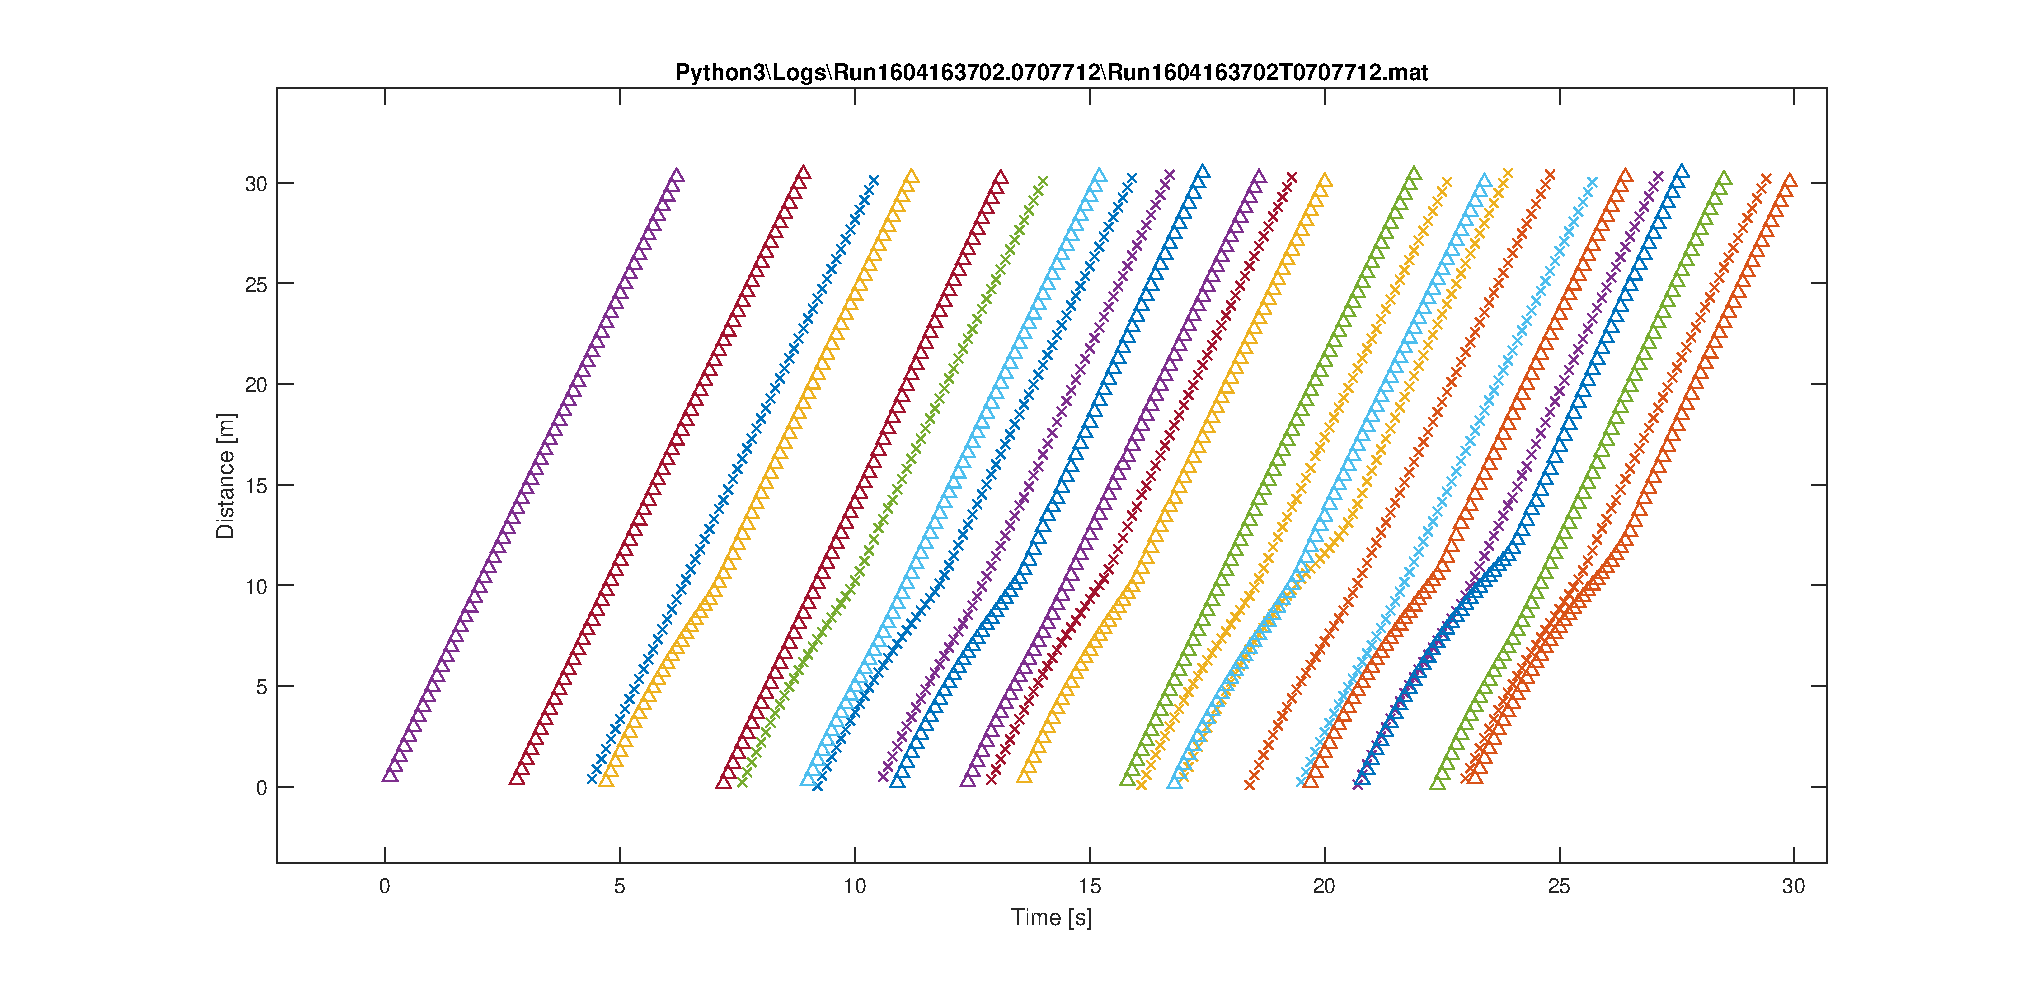
\includegraphics[width=1.0\linewidth]{OptimalFIFOTracesT707712-fixed.eps}
	\caption{The position time series for the FIFO Optimal Controller in scenario 1.}
	\label{fig:optimal_fifo_st}       % Give a unique label
\end{figure}
The distance-time plot for the FIFO Optinal Controller is shown in Figure \ref{fig:optimal_fifo_st}. It was able to proceed for the full 30 seconds without any collision as the approach lane did not fill up. This only shows that the throughput of the FIFO optimal control is higher than semaphore method, and is sufficient to meet the demand of $\lambda=0.5$ on each lane, without a queue forming.   

In these two runs the arrival sources were not linked to the occupancy af the approach lane, so if the approach lane fills up, and average speed drops, so the new arrivals can appear right on top of vehicle at the back of the queue, leading to a collision which the interseciton controller is unable to prevent.  This is not a realistic crash situation because in a real site approaching vehicles will detect the back of queue with their front safety sensor and stop in time. 

In Figure \ref{fig:optimal_fifo_st} it can be seen that 24 vehicles pass through the intersection in 30 seconds. This is very close to the upper limit of one vehicle per second determined by on the arrival rate. 

\subsection{Trajectory Comparison with Dynmaic Arrival Pattern, 30 Departures Run}
\label{sec:mutex_arrival_pattern}
To understand more about the performance of the controllers the arrival pattern was linked to the appraoch lane occpancy. Rather than deal with the complexity of speed reductions due to safety sensors, the model was based on a roadmap reservation system which are widely usedin centralized or decentralized form. The capacity of the approach lane (10 metres long) was set to 1 AGV. If the static arrival pattern suggested an arrival while the lane was full, it entered an arrival queue. At the next simulation time step where the approach lane had capacity, if there was any vehicles in the queue, the first would be introduced to the simulation at the start of the approach lane with zero speed (as opposed to the random arrivals, which enter the lane at full speed).  
\begin{figure}
	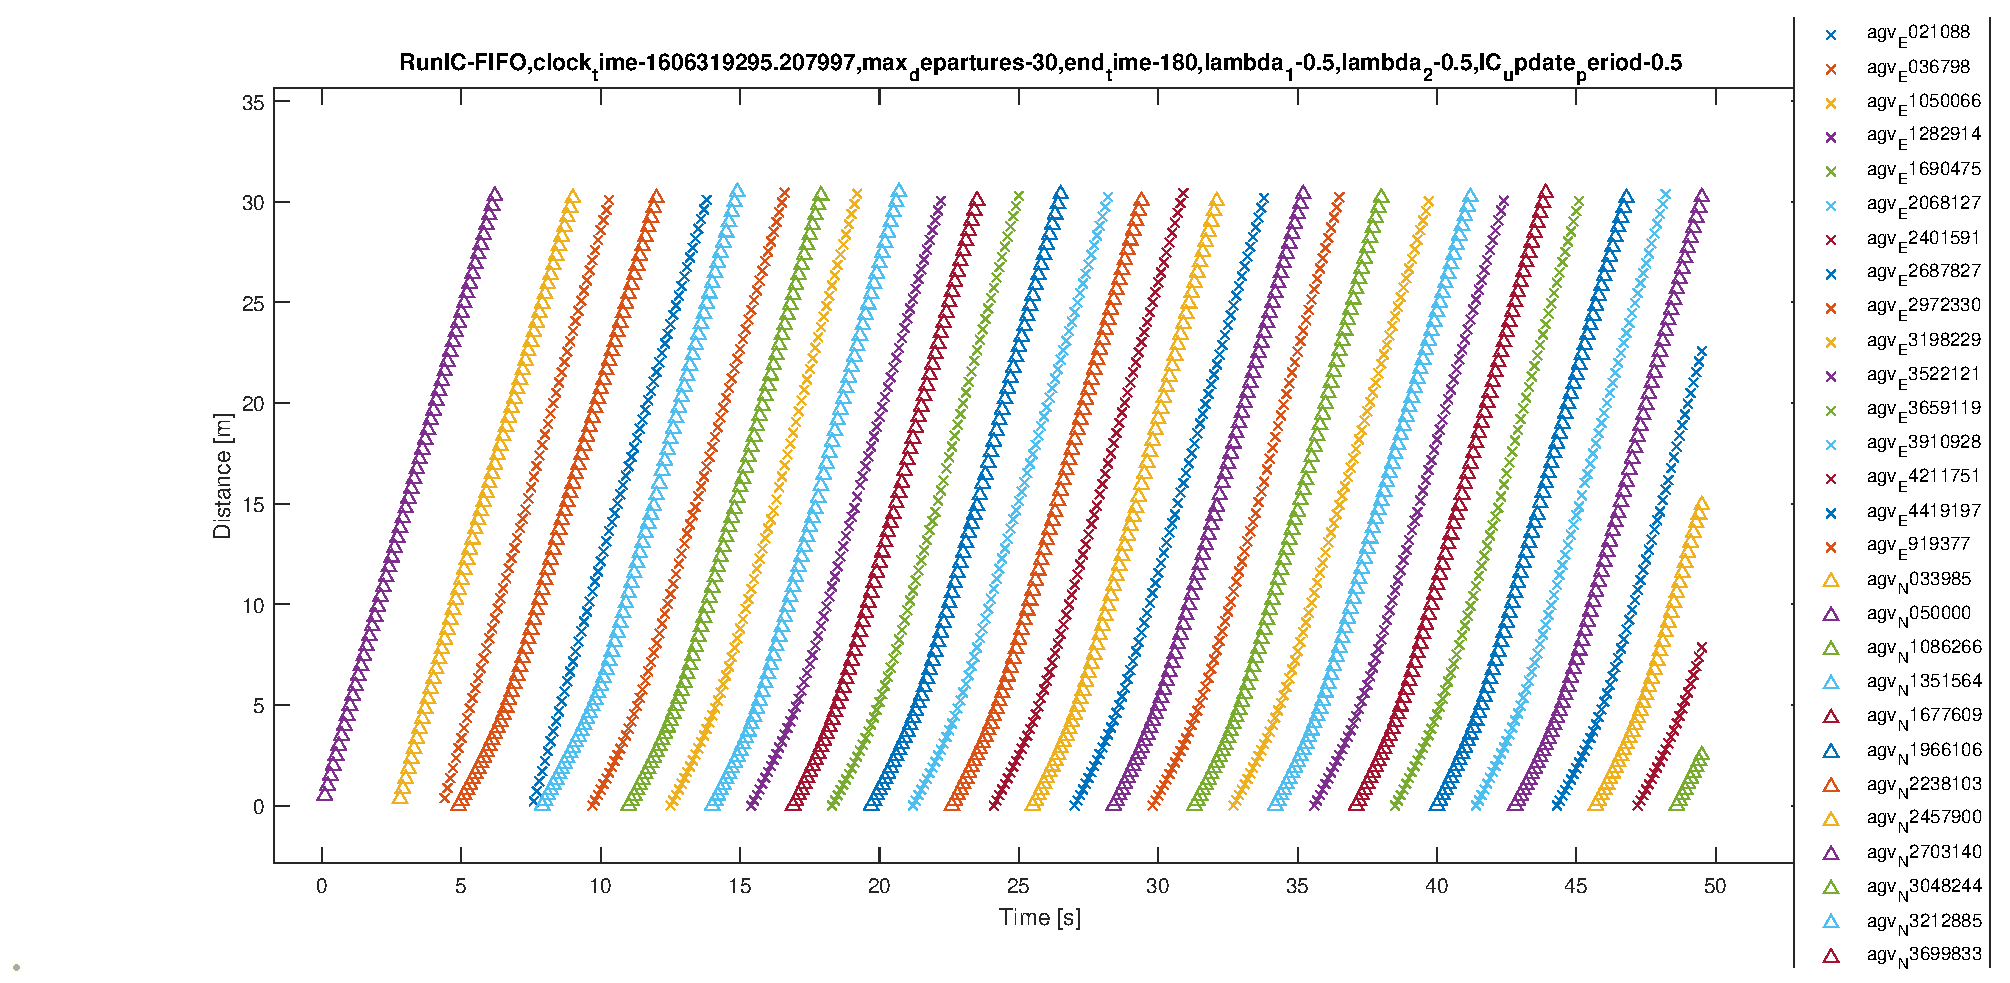
\includegraphics[width=1.0\linewidth]{distance-time-FIFO-HighLatency-HighTraffic.eps}
	\caption{The position time series for the FIFO Optimal Controller in the High Traffic High Latency Scenario}
	\label{fig:optimal_fifo_st_HL_HT}       % Give a unique label
\end{figure}
\begin{figure}
	\includegraphics[width=1.0\linewidth]{Sempahore-716956HighTraffic-HighLatency.eps}
	\caption{The position time series for the Semaphore Controller in the High Traffic High Latency Scenario.}
	\label{fig:semaphore_st_HL_HT}       % Give a unique label
\end{figure}

With arrival lane capacity of one AGV, 30 AGVs were able to cross the intersection in 82.3 seconds with the semaphore control. With FIFO optimal control this was reduced to 49.6 seconds. This is a reduction of 39.7\%, entirely due to centralized speed choice, as both used FIFO ordering. The centralized optimal FIFO controller is able to predict when the conflict will become unoccupied, so following vehicles don't need to slow down as much as with Semaphore control. 

The free flow time to cross 30 metres at maximum speed of 5 metres per second is six seconds. The mean travel time across the Semaphore controlled intersection was 309.1, indicating a delay of 309.1/30 - 6 = 4.30 seconds. The delay due to the FIFO Controlled intersection was 195.1/30 - 6 = 0.50s. This dramatic reduction might be expected given the objective for the FIFO optimal method was to minimise total travel time.   

\subsection{Energy Consumption}
The use of an approach speeds minimising total travel time increases the energy consumption per vehicle as shown in Table \ref{tab:energy_res}. The extra information about the departure time of leading vehicles should lead to reduced energy expense slowing down. As total energy usage (and therefore usage per vehicle) actually increase, and air resistance was not considered,  it suggests the higher average speeds reduce the efficiency of the motor.

\begin{table}
	\begin{tabular}{|c|c|c|}
		\hline
		& Semaphore & FIFO Optimal \\
		\hline
		Total Electrical Energy (MJ) & 542.310& 641.170\\
		Total Mechanical Energy (MJ) & 61.549& 68.448\\
		Completion Time (s) & 82.3 & 49.6\\
		Total Travel Time (s) & 309.1 & 195.1 \\
		\hline
	\end{tabular}
	\label{tab:energy_res}
	\caption{Energy and Completion Time Results }
\end{table}

\begin{figure}
	\includegraphics[width=1.0\linewidth]{agv_e_021088_power_-FIFO-HighLatency-HighTraffic.eps}
	\caption{The power dissipated over time for one AGV under FIFO control.}
	\label{fig:021088power}       % Give a unique label
\end{figure}
\begin{figure}
	\includegraphics[width=0.45\linewidth]{agv_e_021088_power_-FIFO-HighLatency-HighTraffic_zoom_out.eps}
	\caption{Spurious data points of the power dissipated over time for one AGV under FIFO control.}
	\label{fig:021088power_spurious}       % Give a unique label
\end{figure}

\begin{figure}
	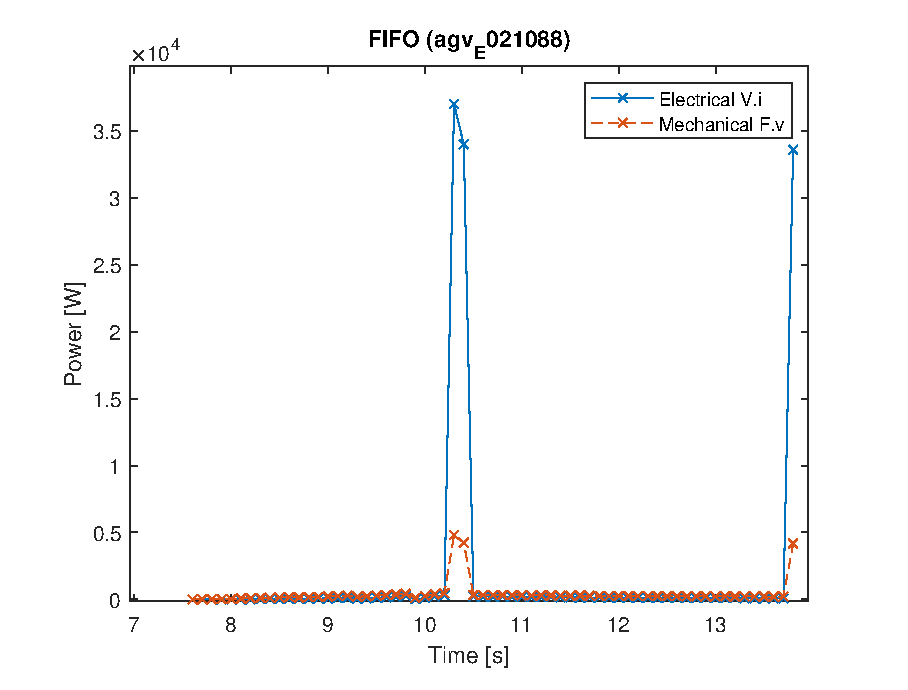
\includegraphics[width=1.0\linewidth]{agv_e_021088_power_-FIFO-HighLatency-HighTraffic-recalc.eps}
	\caption{The electric power was recalculated from the logged value of armature current $i^2$R with a resistance of R=0.001$\omega$. The mechanical power was recalculated using the abs(motive\_force*velocity).}
	\label{fig:recalc_021088power}       % Give a unique label
\end{figure}

\begin{figure}
	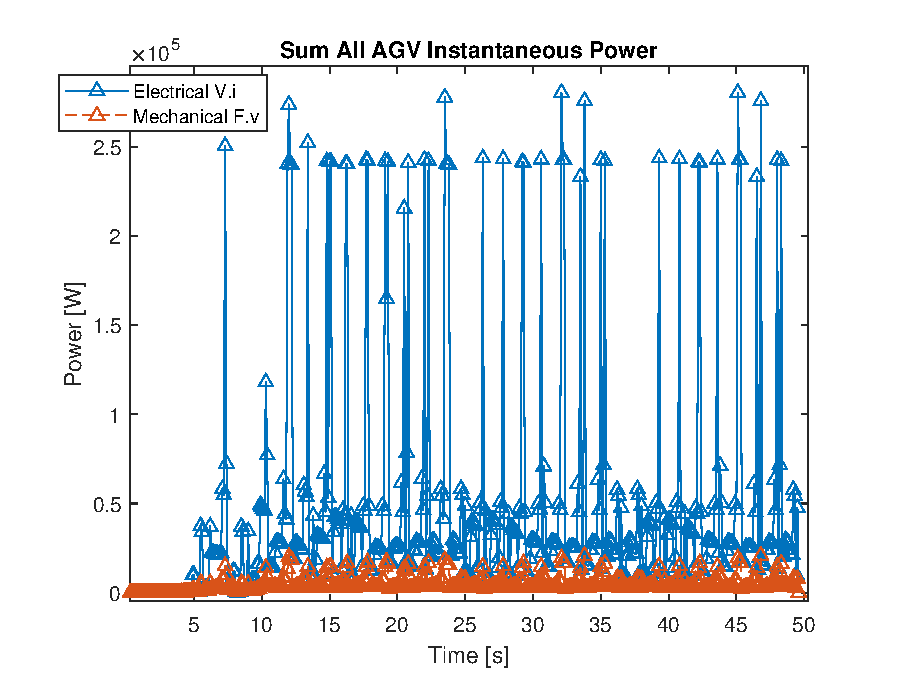
\includegraphics[width=1.0\linewidth]{fifo_power_recalc_sum_all_agv.eps}
	\caption{The power dissipated over time for all AGVs in total under FIFO control.}
	\label{fig:fifo_power_sum}       % Give a unique label
\end{figure}
\begin{figure}
	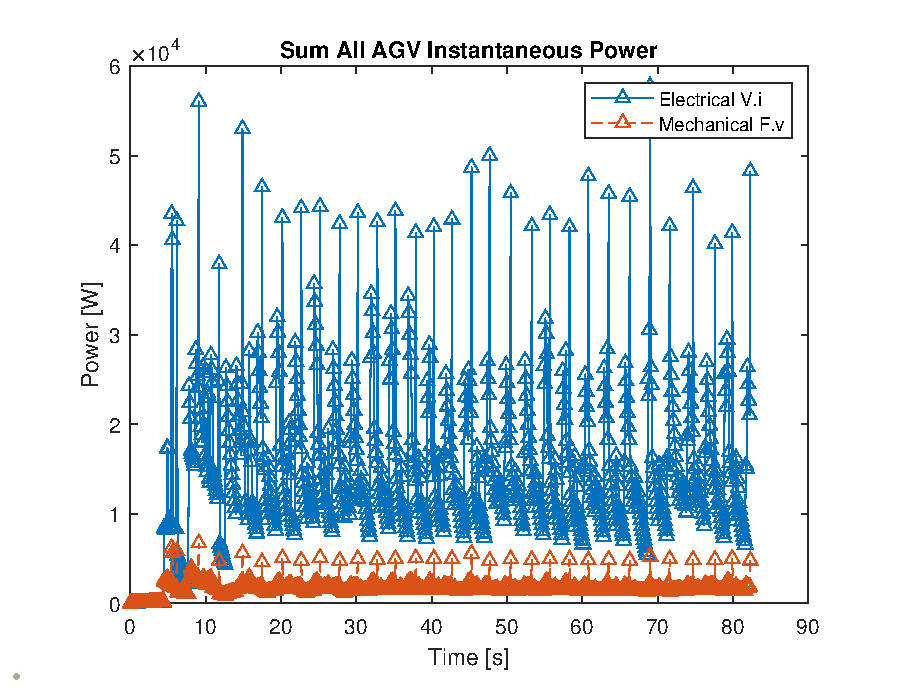
\includegraphics[width=1.0\linewidth]{semaphore_power_recalc_sum_all_agv.eps}
	\caption{The power dissipated over time for all AGVs in total under Semaphore control.}
	\label{fig:semaphore_power_sum}       % Give a unique label
\end{figure}

\bibliographystyle{unsrt}      % basic style, author-year citations - Figure out why citation author lists dont fit in the columns 

\bibliography{roundabouts}   % name your BibTeX data base

\end{document}